\documentclass[11pt]{article}
\usepackage[margin=1in]{geometry}
\usepackage{booktabs}
\usepackage{amsmath, amssymb}
\usepackage{enumitem}
\usepackage[compact]{titlesec}
\usepackage{parskip}
\usepackage{graphicx}
\usepackage{multirow}
\usepackage{float}

\title{L2 Norm Bimodality in CALE Clue Embeddings}
\author{}
\date{}

\begin{document}
\maketitle
\vspace{-4em}

\section*{Overview}

When we embed cryptic clue surfaces using CALE's $\langle t\rangle\langle/t\rangle$ delimiters
($f_\text{clue}$), the L2 norms of the resulting 1024-dimensional vectors are
visibly bimodal, with two peaks at approximately 29.6 and 31.6 (Figure~1,
top row). This report characterizes the bimodality, tests whether it
propagates to our cosine-based research metrics, and documents its behavior
under fine-tuning.

\section*{The Bimodality Is Real and Specific to Clue Context}

We applied a two-criterion bimodality test---$\Delta$BIC~$>$~10 (Kass \&
Raftery 1995) \emph{and} Ashman's $D > 2$ (cleanly separated
components)---to seven $g_\text{stock}$ embedding populations. $\Delta$BIC
alone flags any departure from normality at large $N$; Ashman's $D$ provides
the sample-size-independent effect-size filter.\footnote{$D =
\sqrt{2}\,|\mu_1 - \mu_2| / \sqrt{\sigma_1^2 + \sigma_2^2}$; $D > 2$
corresponds to $<$\,13\% overlap between the two Gaussian components.}

\begin{table}[h]
\centering
\begin{tabular}{lrrrll}
\toprule
Population & $N$ & $\Delta$BIC & Ashman's $D$ & Bimodal? \\
\midrule
$f_\text{clue}$ (full) & 239,406 & 28,806 & 2.88 & Yes \\
$f_\text{clue}$ (val only) & 47,933 & 5,726 & 2.88 & Yes \\
$f_\text{wndef}$ (full) & 53,930 & 400 & 1.88 & No \\
$f_\text{wnex}$ (full) & 8,360 & 388 & 2.11 & Yes \\
$f_\text{wndef}$, wnex words & 8,360 & 140 & 2.12 & Yes \\
\bottomrule
\end{tabular}
\end{table}

The $f_\text{clue}$ distribution passes both criteria decisively
($D = 2.88$). The $f_\text{wndef}$ vocabulary embeddings---the same words,
decontextualized---fail ($D = 1.88$; Figure~1, middle row), confirming that the
bimodality arises from clue context, not from the words themselves.

\begin{figure}[H]
\centering
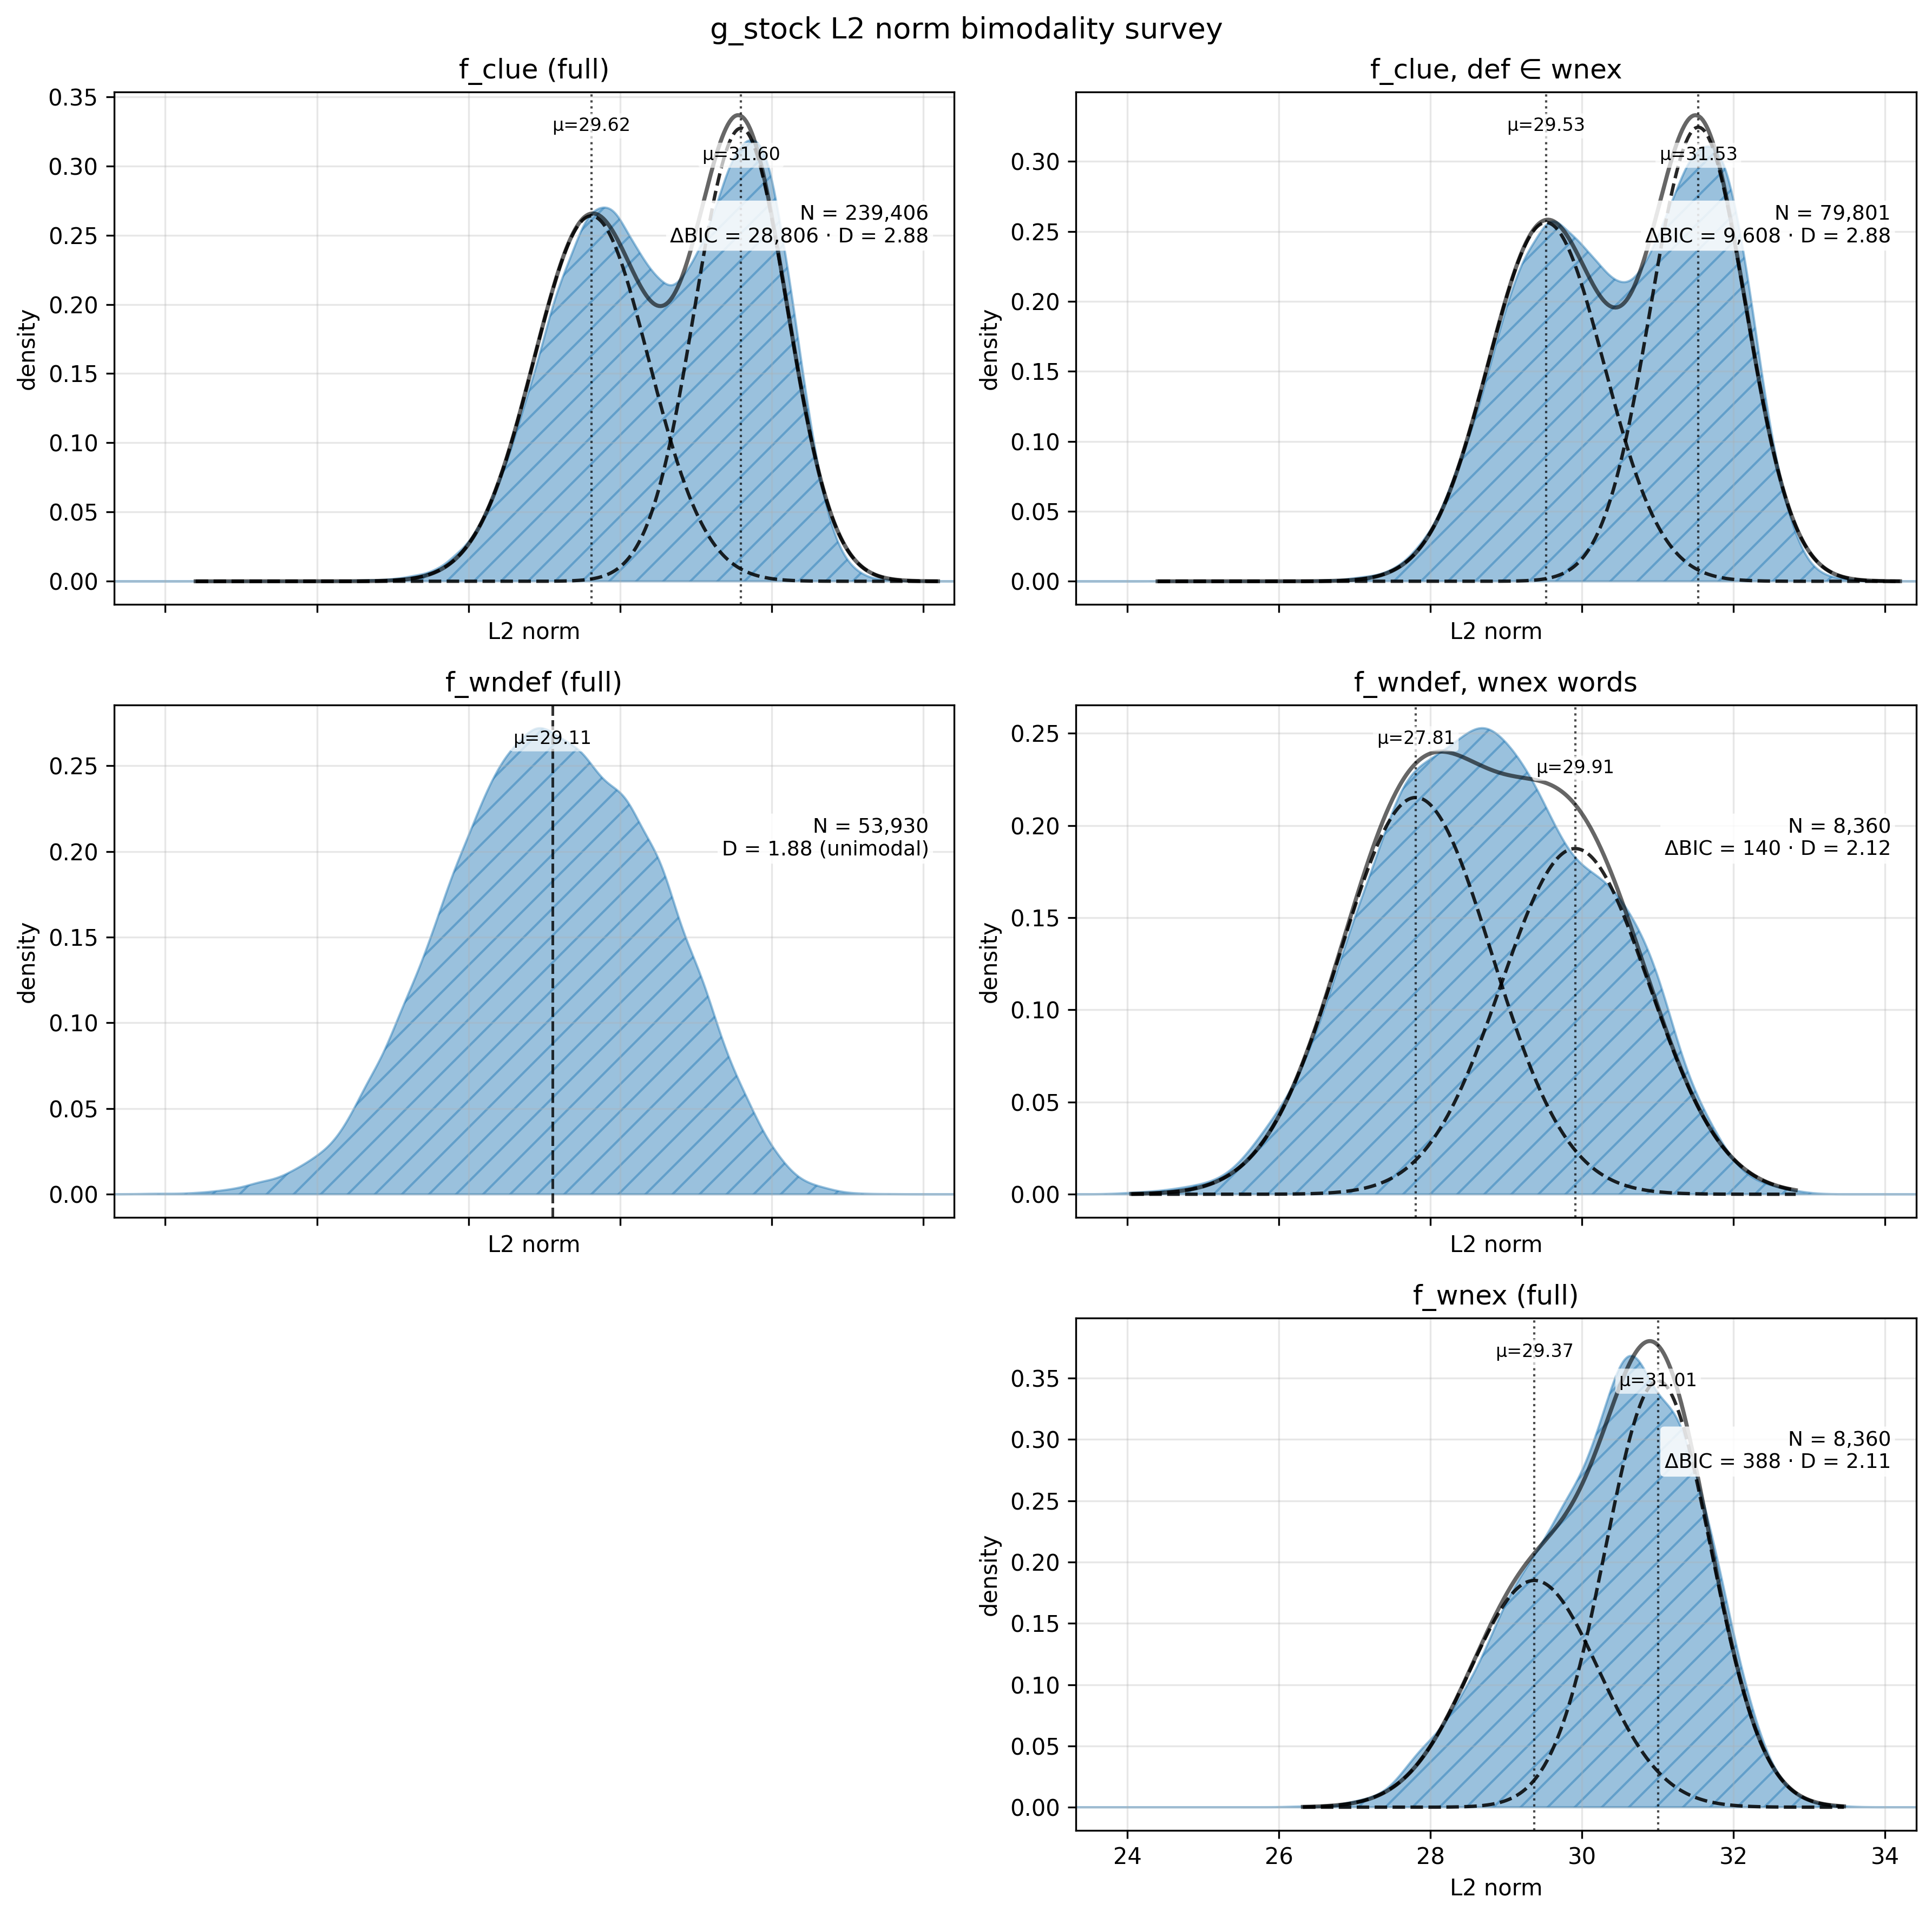
\includegraphics[width=\textwidth]{../figures/norm_bimodality_survey_gstock.png}
\caption{\small L2 norm distributions for $g_\text{stock}$ embeddings across five
populations. Bimodal populations receive 2-component GMM overlays with annotated
component means; unimodal populations show a single mean line. Left column:
full datasets; right column: restricted to the 8,360 words in the wnex
vocabulary, isolating phrase construction from vocabulary composition. The
$f_\text{clue}$ bimodality (top) persists even on the wnex-restricted subset,
while $f_\text{wndef}$ for the same words (middle right) shows a weaker,
less-separated split ($D = 2.12$ vs.\ 2.88).}
\end{figure}

\section*{What Modulates the Bimodality}

\textbf{Definition position.} Whether the tagged definition word appears at
the start or end of the clue surface does not create or destroy the
bimodality---both subsets show two modes at the same locations
($\mu_1 \approx 29.6$, $\mu_2 \approx 31.6$). What changes is the
\emph{balance}: start-of-surface definitions weight the upper mode more
heavily ($\pi_\text{upper} = 0.57$), while end-of-surface definitions weight
the lower mode ($\pi_\text{lower} = 0.59$). The overall distribution looks
bimodal because these two subsets superimpose with different mixture weights.

\textbf{Not the word, not surface features.} An intraclass correlation
(ICC(1,1)\,$=$\,0.14) on per-word $f_\text{clue}$ norms confirms that most
variance is within-word, not between-word: the same definition word receives
different norms in different clues. Cross-format Spearman correlations between
mean $f_\text{clue}$ norm and $f_\text{wndef}$ norm ($\rho = 0.26$) or
$f_\text{wnex}$ norm ($\rho = 0.21$) are weak. A 15-feature regression on
surface properties (token counts, definition position, punctuation, nine
wordplay-type flags) achieves $R^2 = 0.041$---96\% of the variance is
unexplained by any observable text property we tested. The bimodality reflects
something about how CALE's attention mechanism interacts with clue context at
a level deeper than surface tokenization.

\section*{Magnitude Only, Not Direction}

The bimodality is strictly a magnitude phenomenon. A pairwise cosine analysis
on 50,000 pairs of unit-normalized $f_\text{clue}$ embeddings produces a
unimodal distribution (mean cosine $= 0.318$). Splitting embeddings at the
median norm and computing the cosine between the two halves' centroid
directions gives 0.978---the lower-norm and upper-norm groups point in
essentially the same direction.

\section*{No Propagation to Cosine Metrics}

Since our research metric is cosine similarity, the practical question is
whether the norm bimodality confounds the ATE.  Stratifying validation clues
by norm group shows nearly identical $T\!=\!1$ cosine similarity (lower:
0.523, upper: 0.519) and ATE (lower: $-0.053$, upper: $-0.047$). The
Spearman correlation between $f_\text{clue}$ norm and ATE is 0.019. L2-based
$T\!=\!1$ distances \emph{do} differ across norm groups (28.2 vs.\ 29.5),
as expected---but this does not leak into cosine. The bimodality and
misdirection are independent phenomena.

\section*{Fine-Tuning Eliminates the Bimodality}

Under $g_1$, global norm compression collapses both modes. The component
separation shrinks from $\Delta\mu \approx 2.0$ (g\_stock) to
$\Delta\mu \approx 0.9$ ($g_1$), and the overall standard deviation drops
from 1.20 to 0.74. The position-dependent mixture-weight pattern disappears.
This is consistent with the general compression documented in the $g_1$
evaluation: fine-tuning contracted the embedding space uniformly, erasing
the magnitude structure that $g_\text{stock}$ maintained.

\section*{Implications}

The $f_\text{clue}$ norm bimodality is a genuine feature of how
$g_\text{stock}$ represents clue-contextualized words---contextual, not
lexical, and driven by factors below the surface-feature level. It does not
confound cosine-based analyses: ATE measurements are unaffected. L2-based
analyses of $g_\text{stock}$ $f_\text{clue}$ embeddings should be interpreted
with the bimodality in mind, though in practice we report cosine throughout.
Under $g_1$ (or any future fine-tuned model exhibiting similar compression),
the concern does not arise.

\end{document}
